\section{Introduction}

\subsection{Motivation}


Since 60 years ago, MADALINE\cite{adaline}, the first artificial neural network application, predicted the bit streams traversing a phone line, the interest around artificial neural network and artificial intelligence (AI) has grown continuously; see Fig.~\ref{fig:ai-papers}. Apart from the research in the academia, enterprise neural network applications has also increased significantly over these years including automatic speech recognition\cite{yu2016automatic}, self-driving car\cite{maqueda2018event}. This trend was predicted to continue at least by the end of 2025 \cite{ai-invest}. \\

\begin{figure}[!ht]
   \centering
   \begin{subfigure}[b]{0.9\textwidth}
       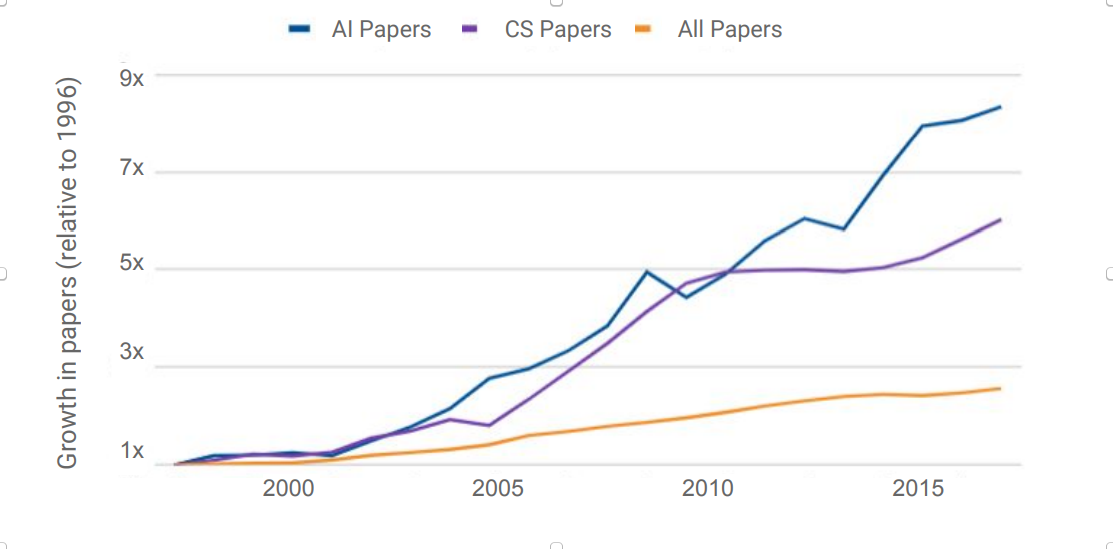
\includegraphics[width=\textwidth]{figures/ai_paper.png}
       \caption{AI papers published per year (image from \cite{ai-papers}).The trend has shown that by the end of 2020, there would be around 8 times more AI academic papers than 1995.}
       \label{fig:ai-papers}
   \end{subfigure}
      ~
   \centering
   \begin{subfigure}[b]{0.9\textwidth}
       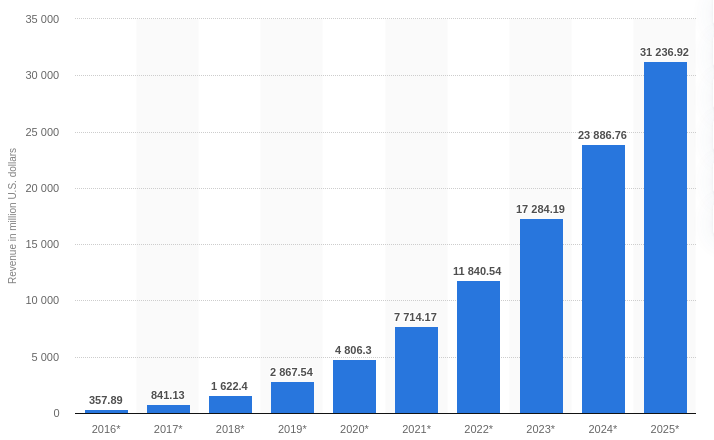
\includegraphics[width=\textwidth]{figures/ai_enterprise.png}
       \caption{Enterprise AI market revenue 2016-2025 (image from \cite{ai-proj}). }
       \label{fig:ai-proj}
   \end{subfigure}%
\end{figure}

To accelerate the field of neuroscience, computing and brain-related medical research, some funding has been allocate to the Human Brain Project (HBP) \cite{hbp}. The HBP project has been broke down to several sub-project. One of them is to build a novel computer with a design inspired by the human brain, which finally led to the Spiking Neural Network Architecture (SpiNNaker) project and a million-core machine (seen in Fig.~\ref{fig:cluster}). Correspondingly, Under the SpiNNaker project, researchers also build a suite of software to support the SpiNNaker hardware and software development.\\

\begin{figure}[!tb]
   \centering
       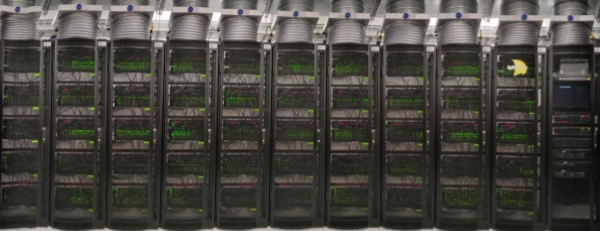
\includegraphics[width=0.7\textwidth]{figures/cluster.png}
       \caption{The 500,000-core SpiNNaker \textit{102} machine at the University of Manchester (image from \cite{spinn-core}).}
       \label{fig:cluster}
\end{figure}


Nowadays, the amount of data has grown increasing large, traditional computer architectures do not scale as the Moore's law \cite{schaller1997moore}. While parallelism is regarded as an option to keep the scaling, the SpiNNaker hardware was designed to be massively distributed and parallel. Thus the SpiNNaker hardware has the potential to be used as a parallel computing solution. As opposite to the traditional hardware, SpiNNaker has the following hardware features:

\begin{itemize}
\item \textbf{Manycore architecture}: though modern CPUs start to have multiple cores to gain some parallelism, the number of cores in a CPU is usually less than 10. On the opposite, a type Spinn-5 SpiNNaker board has 48 chips, which contains hundreds of ARM cores \cite{5th-summit}. Though there are more cores, because of the medium-performance (only 200MHz) ARM968 cores, the energy consumption stays relatively low.

\item \textbf{Communication model}: the SpiNNaker cores communicate by sending message via UDP/IP \cite{ws6} and UDP/IP do not guarantee the delivery. Though it is the developers' responsibility to make sure the correctness, the developers do not need to worry about the dead-lock. It is designed as so because in a real human brain a neuron does not get any an acknowledgement when the communication is done \cite{spinnaker}.

\item \textbf{Communication throughput}: extra performance might be gain from the reduce of the message size and more message can be process in the same amount of time\cite{furber2012overview}. Their link can transfer up to 31.25M byte/s, which means the links can handle 3M packets per second \cite{ws6}.\\
\end{itemize}

Some further background information about the SpiNNaker platform would be covered in section \ref{sec:bg}. \\

In a word, the SpiNNaker has the full potential as a supercomputer. \\
 
On the other side, Computational fluid dynamics (CFD) is a science that, with the help of digital computers, produces quantitative predictions of fluid-flow phenomena based on the conservation laws (conservation of mass, momentum, and energy) governing fluid motion \cite{thelbmbible}. It help us to to solve real-world engineering problems, including aerospace engineering, meteorology, etc. However, CFD algorithm usually involve heavy computation. To get the simulation result in affordable time, scientists and engineers need to accelerate the simulation. Therefore, parallel computers including some supercomputers are heavily used for CFD simulation.\\

Lattice Boltzmann method (more about LBM at \ref{sec:lbmb}) is a CFD model which is recognized\cite{lbmmbook} as: (1) easy to apply to complex domain (2) No need to solve the Laplace equation (3) More importantly for this project, being naturally adapted to parallel processing due to the locality and explicit nature of the method. Due to its (3) nature, many parallel techniques are applied to accelerate the LBM simulation, including MPI\cite{he1999three}, OpenMP\cite{massaioli2002achieving} and GPGPU\cite{rogers1990upwind}, etc. \\

As we discussed above, the SpiNNaker has the ability to compute in massively parallel. Thus, there is a perfect match between the SpiNNaker and the lattice Boltzmann method. It is promising that we can get high performance and scalability in term of speed with SpiNNaker's low energy-consumption cores on the LBM simulation tasks, which is also the motivation behind this project.  \\




\subsection{Objectives} \label{sec:Obj}

Firstly, we can define our objective of this projects as follow:\\

\begin{quote}
\textit{Implementing a basic lattice Boltzmann method simulation on the SpiNNaker platform; and investigate its speed performance and scalability. \\
}\end{quote}

% KS: In point one there are two separate points which should be discussed seaparately. First, there is the implementation of the algirthm. Second, there
% is the use of a standard test problem to check that the implementation is
% working correctly. A wide range of test problems could be used.

% KS: There needs to be more here. It's not just a question of implementation. There
% needs to be some critical evaluation of ease-of-use, performance, and so on. 
% to add to KS. you need to discuss how your going to compare. speed, scale? energy? accuracy?

To break down the mission, we firstly need to implement a basic lattice Boltzmann method on the SpiNNaker. Even before that, we need a standard implementation on CPU, which can be more easily to understand and porting the algorithm; and we can also further evaluate the correctness, accuracy and compare the performance with this CPU implementation.\\

Secondly, we need to choose a pre-defined problem as the test problem from a wide range of the problems. As the test problem, it need to be simple, generic and easy to check the correctness. To choose it, we take LBM model and the boundary condition into consideration, and, finally, a two dimensions and nine vectors (D2Q9) model with a periodic condition problem described by Minion and Brown \cite{minion1997performance} was chosen. It is simple -- it has two dimensions instead of three, generic -- nine vectors need reasonable communication, and easy to check the correctness -- with the mentioned initial condition, there will be a turbulence in a fix step and we can check it.\\

Finally, after implementing the simulation on SpiNNaker, we will to evaluate correctness and accuracy the simulation result by compare the numbers in quantitatively. After we confirm the correctness, them some experiment would be focus on optimization the communication and bench mark the result with the standard CPU implementation on speed-ups and scalability.\\

\subsection{Project Overview}

The work of this project are threefold:\\

\begin{itemize}
\item \textbf{A simple lattice Boltzmann implementation on CPU}: we firstly built a standard serial implementation of a pre-defined lattice Boltzmann scenario described by Minion and Brown \cite{minion1997performance}; see Subsection \ref{sec:ip}. \\

\item \textbf{A simple lattice Boltzmann implementation on SpiNNaker:} after we implemented the simulation on CPU, we used the CPU implementation as a reference to implement the same simulation on SpiNNaker platform with some of the SpiNNaker software development kit; See Section \ref{sec:dail}\\

\item \textbf{An investigation on the speed performance and scalability}: we demonstrate that lattice Boltzmann on SpiNNaker platform offers better speed performance in some large scale when compared to CPU and it also has a good scalability on weak-scaling. We bench-marked two implementations of the lattice Boltzmann method scenario: the first one is the standard implementation of on Cirrus and second one is a implementation on SpiNNaker mentioned above. The observation shows that lattice Boltzmann program can gain 5x speed-up in terms of speed over a certain scale; See Section \ref{sec:eval}.
\end{itemize}


